\documentclass[1p]{elsarticle_modified}
%\bibliographystyle{elsarticle-num}

%\usepackage[colorlinks]{hyperref}
%\usepackage{abbrmath_seonhwa} %\Abb, \Ascr, \Acal ,\Abf, \Afrak
\usepackage{amsfonts}
\usepackage{amssymb}
\usepackage{amsmath}
\usepackage{amsthm}
\usepackage{scalefnt}
\usepackage{amsbsy}
\usepackage{kotex}
\usepackage{caption}
\usepackage{subfig}
\usepackage{color}
\usepackage{graphicx}
\usepackage{xcolor} %% white, black, red, green, blue, cyan, magenta, yellow
\usepackage{float}
\usepackage{setspace}
\usepackage{hyperref}

\usepackage{tikz}
\usetikzlibrary{arrows}

\usepackage{multirow}
\usepackage{array} % fixed length table
\usepackage{hhline}

%%%%%%%%%%%%%%%%%%%%%
\makeatletter
\renewcommand*\env@matrix[1][\arraystretch]{%
	\edef\arraystretch{#1}%
	\hskip -\arraycolsep
	\let\@ifnextchar\new@ifnextchar
	\array{*\c@MaxMatrixCols c}}
\makeatother %https://tex.stackexchange.com/questions/14071/how-can-i-increase-the-line-spacing-in-a-matrix
%%%%%%%%%%%%%%%

\usepackage[normalem]{ulem}

\newcommand{\msout}[1]{\ifmmode\text{\sout{\ensuremath{#1}}}\else\sout{#1}\fi}
%SOURCE: \msout is \stkout macro in https://tex.stackexchange.com/questions/20609/strikeout-in-math-mode

\newcommand{\cancel}[1]{
	\ifmmode
	{\color{red}\msout{#1}}
	\else
	{\color{red}\sout{#1}}
	\fi
}

\newcommand{\add}[1]{
	{\color{blue}\uwave{#1}}
}

\newcommand{\replace}[2]{
	\ifmmode
	{\color{red}\msout{#1}}{\color{blue}\uwave{#2}}
	\else
	{\color{red}\sout{#1}}{\color{blue}\uwave{#2}}
	\fi
}

\newcommand{\Sol}{\mathcal{S}} %segment
\newcommand{\D}{D} %diagram
\newcommand{\A}{\mathcal{A}} %arc


%%%%%%%%%%%%%%%%%%%%%%%%%%%%%5 test

\def\sl{\operatorname{\textup{SL}}(2,\Cbb)}
\def\psl{\operatorname{\textup{PSL}}(2,\Cbb)}
\def\quan{\mkern 1mu \triangleright \mkern 1mu}

\theoremstyle{definition}
\newtheorem{thm}{Theorem}[section]
\newtheorem{prop}[thm]{Proposition}
\newtheorem{lem}[thm]{Lemma}
\newtheorem{ques}[thm]{Question}
\newtheorem{cor}[thm]{Corollary}
\newtheorem{defn}[thm]{Definition}
\newtheorem{exam}[thm]{Example}
\newtheorem{rmk}[thm]{Remark}
\newtheorem{alg}[thm]{Algorithm}

\newcommand{\I}{\sqrt{-1}}
\begin{document}

%\begin{frontmatter}
%
%\title{Boundary parabolic representations of knots up to 8 crossings}
%
%%% Group authors per affiliation:
%\author{Yunhi Cho} 
%\address{Department of Mathematics, University of Seoul, Seoul, Korea}
%\ead{yhcho@uos.ac.kr}
%
%
%\author{Seonhwa Kim} %\fnref{s_kim}}
%\address{Center for Geometry and Physics, Institute for Basic Science, Pohang, 37673, Korea}
%\ead{ryeona17@ibs.re.kr}
%
%\author{Hyuk Kim}
%\address{Department of Mathematical Sciences, Seoul National University, Seoul 08826, Korea}
%\ead{hyukkim@snu.ac.kr}
%
%\author{Seokbeom Yoon}
%\address{Department of Mathematical Sciences, Seoul National University, Seoul, 08826,  Korea}
%\ead{sbyoon15@snu.ac.kr}
%
%\begin{abstract}
%We find all boundary parabolic representation of knots up to 8 crossings.
%
%\end{abstract}
%\begin{keyword}
%    \MSC[2010] 57M25 
%\end{keyword}
%
%\end{frontmatter}

%\linenumbers
%\tableofcontents
%
\newcommand\colored[1]{\textcolor{white}{\rule[-0.35ex]{0.8em}{1.4ex}}\kern-0.8em\color{red} #1}%
%\newcommand\colored[1]{\textcolor{white}{ #1}\kern-2.17ex	\textcolor{white}{ #1}\kern-1.81ex	\textcolor{white}{ #1}\kern-2.15ex\color{red}#1	}

{\Large $\underline{11a_{142}~(K11a_{142})}$}

\setlength{\tabcolsep}{10pt}
\renewcommand{\arraystretch}{1.6}
\vspace{1cm}\begin{tabular}{m{100pt}>{\centering\arraybackslash}m{274pt}}
\multirow{5}{120pt}{
	\centering
	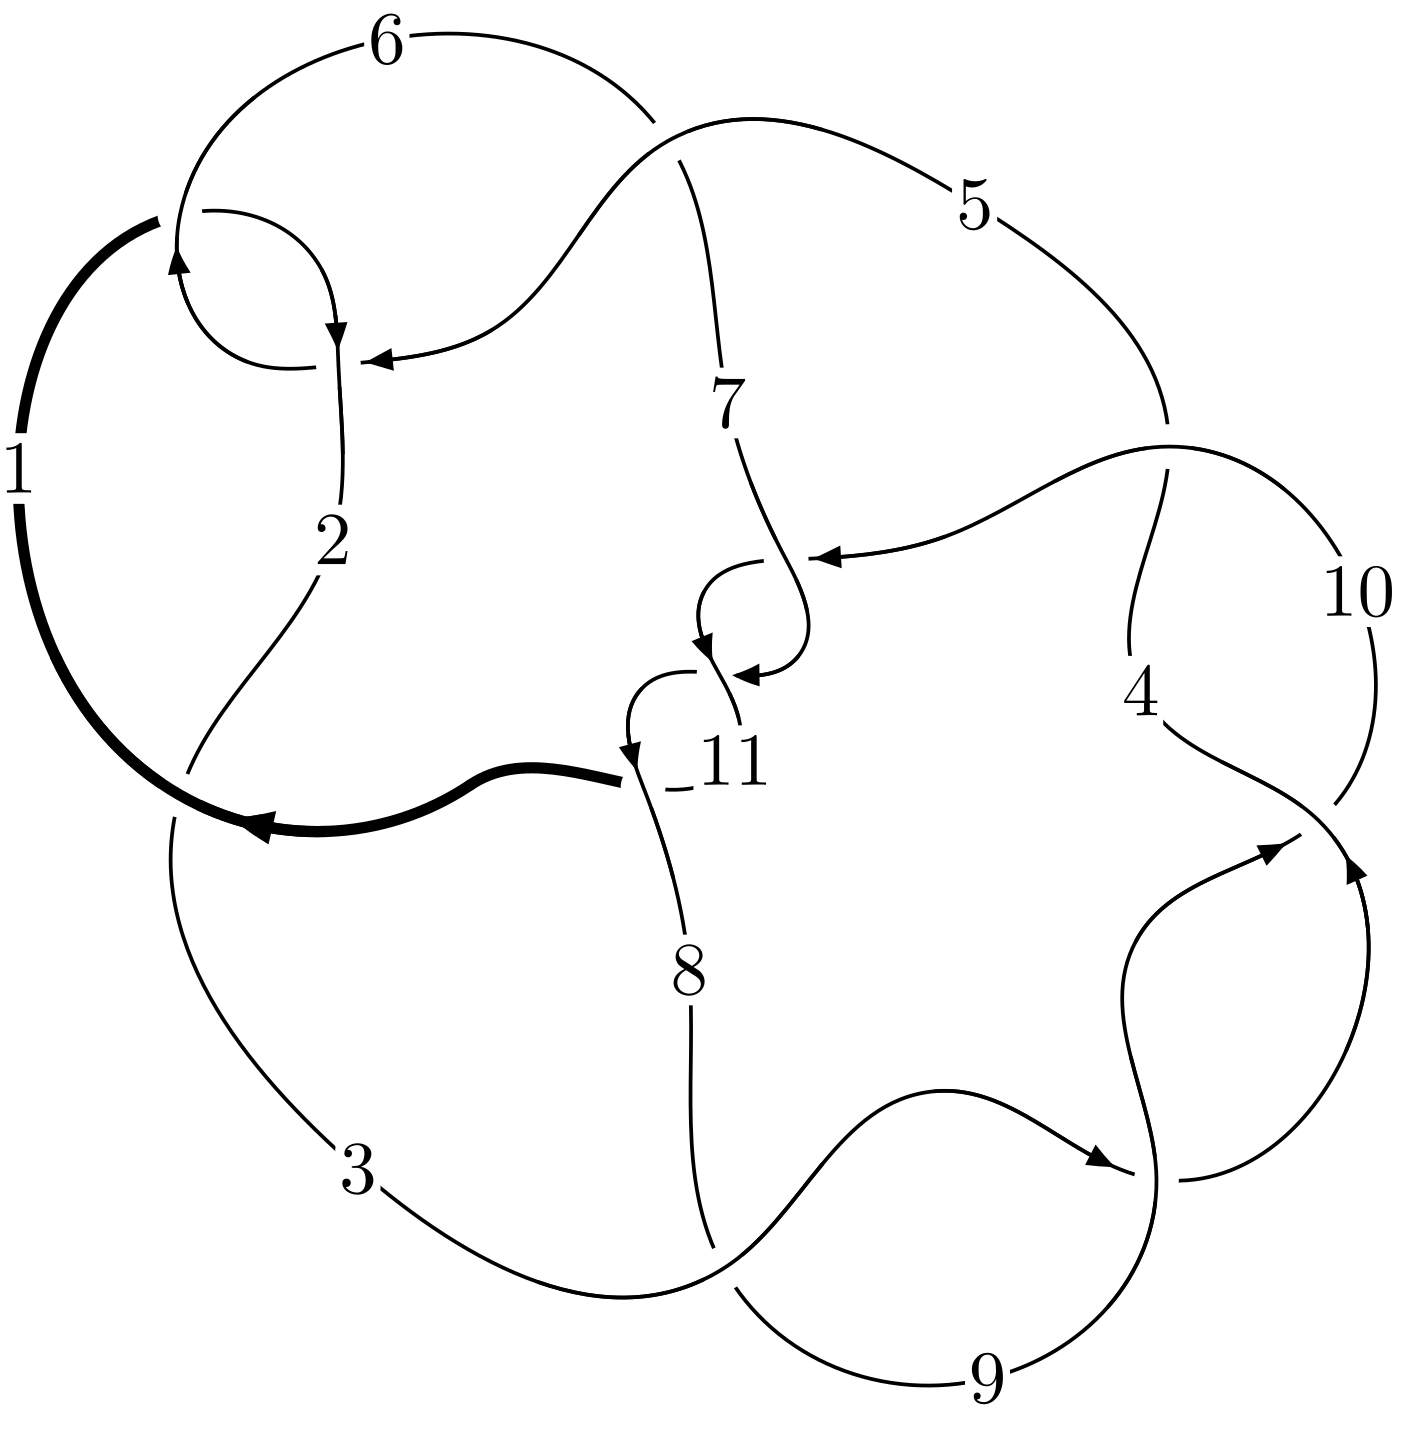
\includegraphics[width=112pt]{../../../GIT/diagram.site/Diagrams/png/391_11a_142.png}\\
\ \ \ A knot diagram\footnotemark}&
\allowdisplaybreaks
\textbf{Linearized knot diagam} \\
\cline{2-2}
 &
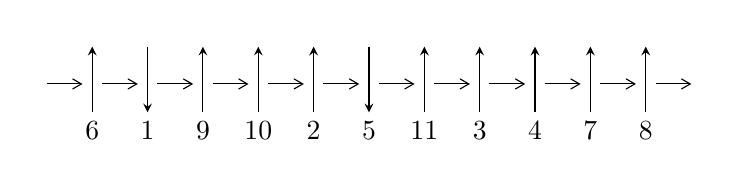
\begin{tikzpicture}[x=20pt, y=17pt]
	% nodes
	\node (C0) at (0, 0) {};
	\node (C1) at (1, 0) {};
	\node (C1U) at (1, +1) {};
	\node (C1D) at (1, -1) {6};

	\node (C2) at (2, 0) {};
	\node (C2U) at (2, +1) {};
	\node (C2D) at (2, -1) {1};

	\node (C3) at (3, 0) {};
	\node (C3U) at (3, +1) {};
	\node (C3D) at (3, -1) {9};

	\node (C4) at (4, 0) {};
	\node (C4U) at (4, +1) {};
	\node (C4D) at (4, -1) {10};

	\node (C5) at (5, 0) {};
	\node (C5U) at (5, +1) {};
	\node (C5D) at (5, -1) {2};

	\node (C6) at (6, 0) {};
	\node (C6U) at (6, +1) {};
	\node (C6D) at (6, -1) {5};

	\node (C7) at (7, 0) {};
	\node (C7U) at (7, +1) {};
	\node (C7D) at (7, -1) {11};

	\node (C8) at (8, 0) {};
	\node (C8U) at (8, +1) {};
	\node (C8D) at (8, -1) {3};

	\node (C9) at (9, 0) {};
	\node (C9U) at (9, +1) {};
	\node (C9D) at (9, -1) {4};

	\node (C10) at (10, 0) {};
	\node (C10U) at (10, +1) {};
	\node (C10D) at (10, -1) {7};

	\node (C11) at (11, 0) {};
	\node (C11U) at (11, +1) {};
	\node (C11D) at (11, -1) {8};
	\node (C12) at (12, 0) {};

	% arrows
	\draw[->,>={angle 60}]
	(C0) edge (C1) (C1) edge (C2) (C2) edge (C3) (C3) edge (C4) (C4) edge (C5) (C5) edge (C6) (C6) edge (C7) (C7) edge (C8) (C8) edge (C9) (C9) edge (C10) (C10) edge (C11) (C11) edge (C12) ;	\draw[->,>=stealth]
	(C1D) edge (C1U) (C2U) edge (C2D) (C3D) edge (C3U) (C4D) edge (C4U) (C5D) edge (C5U) (C6U) edge (C6D) (C7D) edge (C7U) (C8D) edge (C8U) (C9D) edge (C9U) (C10D) edge (C10U) (C11D) edge (C11U) ;
	\end{tikzpicture} \\
\hhline{~~} \\& 
\textbf{Solving Sequence} \\ \cline{2-2} 
 &
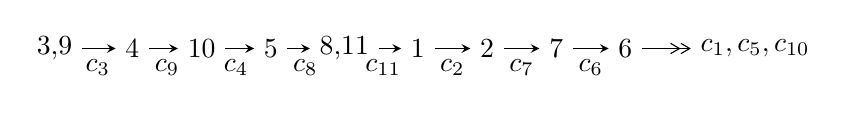
\begin{tikzpicture}[x=25pt, y=7pt]
	% node
	\node (A0) at (-1/8, 0) {3,9};
	\node (A1) at (1, 0) {4};
	\node (A2) at (2, 0) {10};
	\node (A3) at (3, 0) {5};
	\node (A4) at (65/16, 0) {8,11};
	\node (A5) at (41/8, 0) {1};
	\node (A6) at (49/8, 0) {2};
	\node (A7) at (57/8, 0) {7};
	\node (A8) at (65/8, 0) {6};
	\node (C1) at (1/2, -1) {$c_{3}$};
	\node (C2) at (3/2, -1) {$c_{9}$};
	\node (C3) at (5/2, -1) {$c_{4}$};
	\node (C4) at (7/2, -1) {$c_{8}$};
	\node (C5) at (37/8, -1) {$c_{11}$};
	\node (C6) at (45/8, -1) {$c_{2}$};
	\node (C7) at (53/8, -1) {$c_{7}$};
	\node (C8) at (61/8, -1) {$c_{6}$};
	\node (A9) at (10, 0) {$c_{1},c_{5},c_{10}$};

	% edge
	\draw[->,>=stealth]	
	(A0) edge (A1) (A1) edge (A2) (A2) edge (A3) (A3) edge (A4) (A4) edge (A5) (A5) edge (A6) (A6) edge (A7) (A7) edge (A8) ;
	\draw[->>,>={angle 60}]	
	(A8) edge (A9);
\end{tikzpicture} \\ 

\end{tabular} \\

\footnotetext{
The image of knot diagram is generated by the software ``\textbf{Draw programme}" developed by Andrew Bartholomew(\url{http://www.layer8.co.uk/maths/draw/index.htm\#Running-draw}), where we modified some parts for our purpose(\url{https://github.com/CATsTAILs/LinksPainter}).
}\phantom \\ \newline 
\centering \textbf{Ideals for irreducible components\footnotemark of $X_{\text{par}}$} 
 
\begin{align*}
I^u_{1}&=\langle 
-6.36795\times10^{16} u^{34}-7.90337\times10^{16} u^{33}+\cdots+3.65214\times10^{17} b-1.06187\times10^{17},\\
\phantom{I^u_{1}}&\phantom{= \langle  }3.20846\times10^{16} u^{34}+7.33609\times10^{16} u^{33}+\cdots+3.65214\times10^{17} a+5.49062\times10^{17},\;u^{35}- u^{34}+\cdots-12 u-4\rangle \\
I^u_{2}&=\langle 
2 b+2 a+u,\;2 a^2-2 a u-2 a+u+3,\;u^2-2\rangle \\
\\
I^v_{1}&=\langle 
a,\;b- v+1,\;v^2- v+1\rangle \\
\end{align*}
\raggedright * 3 irreducible components of $\dim_{\mathbb{C}}=0$, with total 41 representations.\\
\footnotetext{All coefficients of polynomials are rational numbers. But the coefficients are sometimes approximated in decimal forms when there is not enough margin.}
\newpage
\renewcommand{\arraystretch}{1}
\centering \section*{I. $I^u_{1}= \langle -6.37\times10^{16} u^{34}-7.90\times10^{16} u^{33}+\cdots+3.65\times10^{17} b-1.06\times10^{17},\;3.21\times10^{16} u^{34}+7.34\times10^{16} u^{33}+\cdots+3.65\times10^{17} a+5.49\times10^{17},\;u^{35}- u^{34}+\cdots-12 u-4 \rangle$}
\flushleft \textbf{(i) Arc colorings}\\
\begin{tabular}{m{7pt} m{180pt} m{7pt} m{180pt} }
\flushright $a_{3}=$&$\begin{pmatrix}1\\0\end{pmatrix}$ \\
\flushright $a_{9}=$&$\begin{pmatrix}0\\u\end{pmatrix}$ \\
\flushright $a_{4}=$&$\begin{pmatrix}1\\- u^2\end{pmatrix}$ \\
\flushright $a_{10}=$&$\begin{pmatrix}u\\- u^3+u\end{pmatrix}$ \\
\flushright $a_{5}=$&$\begin{pmatrix}- u^2+1\\u^4-2 u^2\end{pmatrix}$ \\
\flushright $a_{8}=$&$\begin{pmatrix}- u\\u\end{pmatrix}$ \\
\flushright $a_{11}=$&$\begin{pmatrix}-0.0878513 u^{34}-0.200871 u^{33}+\cdots-1.92802 u-1.50340\\0.174362 u^{34}+0.216404 u^{33}+\cdots+2.30563 u+0.290753\end{pmatrix}$ \\
\flushright $a_{1}=$&$\begin{pmatrix}-0.0624444 u^{34}+0.0343900 u^{33}+\cdots-0.357458 u-1.09522\\0.148955 u^{34}-0.0188573 u^{33}+\cdots+0.735065 u-0.117420\end{pmatrix}$ \\
\flushright $a_{2}=$&$\begin{pmatrix}0.00194352 u^{34}+0.344883 u^{33}+\cdots+1.74022 u+2.04509\\-0.0876840 u^{34}-0.158849 u^{33}+\cdots-1.60828 u-0.239291\end{pmatrix}$ \\
\flushright $a_{7}=$&$\begin{pmatrix}0.0878513 u^{34}+0.200871 u^{33}+\cdots+1.92802 u+1.50340\\-0.268809 u^{34}-0.150206 u^{33}+\cdots-1.51044 u-0.864136\end{pmatrix}$ \\
\flushright $a_{6}=$&$\begin{pmatrix}0.0328237 u^{34}-0.0751277 u^{33}+\cdots+0.506093 u+0.865585\\0.00374850 u^{34}-0.0472669 u^{33}+\cdots+0.524988 u-0.0604220\end{pmatrix}$\\ \flushright $a_{6}=$&$\begin{pmatrix}0.0328237 u^{34}-0.0751277 u^{33}+\cdots+0.506093 u+0.865585\\0.00374850 u^{34}-0.0472669 u^{33}+\cdots+0.524988 u-0.0604220\end{pmatrix}$\\&\end{tabular}
\flushleft \textbf{(ii) Obstruction class $= -1$}\\~\\
\flushleft \textbf{(iii) Cusp Shapes $= -\frac{32902895900849614}{91303571055107371} u^{34}+\frac{12004762532282944}{91303571055107371} u^{33}+\cdots+\frac{239783904823467776}{91303571055107371} u+\frac{1365844903778505204}{91303571055107371}$}\\~\\
\newpage\renewcommand{\arraystretch}{1}
\flushleft \textbf{(iv) u-Polynomials at the component}\newline \\
\begin{tabular}{m{50pt}|m{274pt}}
Crossings & \hspace{64pt}u-Polynomials at each crossing \\
\hline $$\begin{aligned}c_{1},c_{5}\end{aligned}$$&$\begin{aligned}
&u^{35}-2 u^{34}+\cdots-2 u+1
\end{aligned}$\\
\hline $$\begin{aligned}c_{2},c_{6}\end{aligned}$$&$\begin{aligned}
&u^{35}+10 u^{34}+\cdots+4 u-1
\end{aligned}$\\
\hline $$\begin{aligned}c_{3},c_{4},c_{8}\\c_{9}\end{aligned}$$&$\begin{aligned}
&u^{35}+u^{34}+\cdots-12 u+4
\end{aligned}$\\
\hline $$\begin{aligned}c_{7},c_{10},c_{11}\end{aligned}$$&$\begin{aligned}
&u^{35}-3 u^{34}+\cdots+7 u+7
\end{aligned}$\\
\hline
\end{tabular}\\~\\
\newpage\renewcommand{\arraystretch}{1}
\flushleft \textbf{(v) Riley Polynomials at the component}\newline \\
\begin{tabular}{m{50pt}|m{274pt}}
Crossings & \hspace{64pt}Riley Polynomials at each crossing \\
\hline $$\begin{aligned}c_{1},c_{5}\end{aligned}$$&$\begin{aligned}
&y^{35}+10 y^{34}+\cdots+4 y-1
\end{aligned}$\\
\hline $$\begin{aligned}c_{2},c_{6}\end{aligned}$$&$\begin{aligned}
&y^{35}+34 y^{34}+\cdots+108 y-1
\end{aligned}$\\
\hline $$\begin{aligned}c_{3},c_{4},c_{8}\\c_{9}\end{aligned}$$&$\begin{aligned}
&y^{35}-45 y^{34}+\cdots+80 y-16
\end{aligned}$\\
\hline $$\begin{aligned}c_{7},c_{10},c_{11}\end{aligned}$$&$\begin{aligned}
&y^{35}-39 y^{34}+\cdots+749 y-49
\end{aligned}$\\
\hline
\end{tabular}\\~\\
\newpage\flushleft \textbf{(vi) Complex Volumes and Cusp Shapes}
$$\begin{array}{c|c|c}  
\text{Solutions to }I^u_{1}& \I (\text{vol} + \sqrt{-1}CS) & \text{Cusp shape}\\
 \hline 
\begin{aligned}
u &= \phantom{-}1.01124\phantom{ +0.000000I} \\
a &= \phantom{-}0.435017\phantom{ +0.000000I} \\
b &= -1.74489\phantom{ +0.000000I}\end{aligned}
 & \phantom{-}5.84048\phantom{ +0.000000I} & \phantom{-}16.2440\phantom{ +0.000000I} \\ \hline\begin{aligned}
u &= \phantom{-}0.842940 + 0.301389 I \\
a &= \phantom{-}0.279499 + 1.063810 I \\
b &= \phantom{-}0.541332 - 0.560583 I\end{aligned}
 & \phantom{-}3.15741 + 4.91553 I & \phantom{-}11.80461 - 7.26359 I \\ \hline\begin{aligned}
u &= \phantom{-}0.842940 - 0.301389 I \\
a &= \phantom{-}0.279499 - 1.063810 I \\
b &= \phantom{-}0.541332 + 0.560583 I\end{aligned}
 & \phantom{-}3.15741 - 4.91553 I & \phantom{-}11.80461 + 7.26359 I \\ \hline\begin{aligned}
u &= -0.046502 + 0.876821 I \\
a &= -0.05406 - 1.61301 I \\
b &= \phantom{-}0.014495 - 0.143542 I\end{aligned}
 & \phantom{-}7.57337 + 3.08858 I & \phantom{-}11.98726 - 2.45837 I \\ \hline\begin{aligned}
u &= -0.046502 - 0.876821 I \\
a &= -0.05406 + 1.61301 I \\
b &= \phantom{-}0.014495 + 0.143542 I\end{aligned}
 & \phantom{-}7.57337 - 3.08858 I & \phantom{-}11.98726 + 2.45837 I \\ \hline\begin{aligned}
u &= -0.924843 + 0.638045 I \\
a &= -0.377611 + 0.218222 I \\
b &= \phantom{-}1.63025 + 0.42363 I\end{aligned}
 & \phantom{-}10.22050 - 8.11783 I & \phantom{-}13.7681 + 6.1510 I \\ \hline\begin{aligned}
u &= -0.924843 - 0.638045 I \\
a &= -0.377611 - 0.218222 I \\
b &= \phantom{-}1.63025 - 0.42363 I\end{aligned}
 & \phantom{-}10.22050 + 8.11783 I & \phantom{-}13.7681 - 6.1510 I \\ \hline\begin{aligned}
u &= -0.855744 + 0.143816 I \\
a &= -0.530278 + 1.121980 I \\
b &= -0.261867 - 0.584427 I\end{aligned}
 & \phantom{-}3.37741 + 0.53913 I & \phantom{-}12.96867 + 0.98562 I \\ \hline\begin{aligned}
u &= -0.855744 - 0.143816 I \\
a &= -0.530278 - 1.121980 I \\
b &= -0.261867 + 0.584427 I\end{aligned}
 & \phantom{-}3.37741 - 0.53913 I & \phantom{-}12.96867 - 0.98562 I \\ \hline\begin{aligned}
u &= \phantom{-}1.002070 + 0.587960 I \\
a &= \phantom{-}0.398952 + 0.208816 I \\
b &= -1.62413 + 0.38544 I\end{aligned}
 & \phantom{-}10.76680 + 1.81479 I & \phantom{-}14.8433 - 1.1672 I\\
 \hline 
 \end{array}$$\newpage$$\begin{array}{c|c|c}  
\text{Solutions to }I^u_{1}& \I (\text{vol} + \sqrt{-1}CS) & \text{Cusp shape}\\
 \hline 
\begin{aligned}
u &= \phantom{-}1.002070 - 0.587960 I \\
a &= \phantom{-}0.398952 - 0.208816 I \\
b &= -1.62413 - 0.38544 I\end{aligned}
 & \phantom{-}10.76680 - 1.81479 I & \phantom{-}14.8433 + 1.1672 I \\ \hline\begin{aligned}
u &= -0.746503 + 0.235179 I \\
a &= -0.327678 + 0.089960 I \\
b &= \phantom{-}1.94693 + 0.30523 I\end{aligned}
 & \phantom{-}2.70500 - 3.34459 I & \phantom{-}11.31994 + 5.51487 I \\ \hline\begin{aligned}
u &= -0.746503 - 0.235179 I \\
a &= -0.327678 - 0.089960 I \\
b &= \phantom{-}1.94693 - 0.30523 I\end{aligned}
 & \phantom{-}2.70500 + 3.34459 I & \phantom{-}11.31994 - 5.51487 I \\ \hline\begin{aligned}
u &= \phantom{-}0.418462 + 0.378689 I \\
a &= \phantom{-}0.176733 + 0.515354 I \\
b &= \phantom{-}0.541640 + 0.031955 I\end{aligned}
 & -1.54201 + 1.37506 I & \phantom{-}2.61836 - 5.92080 I \\ \hline\begin{aligned}
u &= \phantom{-}0.418462 - 0.378689 I \\
a &= \phantom{-}0.176733 - 0.515354 I \\
b &= \phantom{-}0.541640 - 0.031955 I\end{aligned}
 & -1.54201 - 1.37506 I & \phantom{-}2.61836 + 5.92080 I \\ \hline\begin{aligned}
u &= \phantom{-}1.45544 + 0.05665 I \\
a &= \phantom{-}0.731751 + 0.109995 I \\
b &= -1.382100 + 0.064187 I\end{aligned}
 & \phantom{-}6.70444 + 0.15451 I & \phantom{-}13.90887 + 0. I\phantom{ +0.000000I} \\ \hline\begin{aligned}
u &= \phantom{-}1.45544 - 0.05665 I \\
a &= \phantom{-}0.731751 - 0.109995 I \\
b &= -1.382100 - 0.064187 I\end{aligned}
 & \phantom{-}6.70444 - 0.15451 I & \phantom{-}13.90887 + 0. I\phantom{ +0.000000I} \\ \hline\begin{aligned}
u &= -1.48918 + 0.04339 I \\
a &= -1.030150 - 0.268681 I \\
b &= \phantom{-}1.268110 + 0.012077 I\end{aligned}
 & \phantom{-}4.71864 - 2.64789 I & \phantom{-}7.00000 + 4.86854 I \\ \hline\begin{aligned}
u &= -1.48918 - 0.04339 I \\
a &= -1.030150 + 0.268681 I \\
b &= \phantom{-}1.268110 - 0.012077 I\end{aligned}
 & \phantom{-}4.71864 + 2.64789 I & \phantom{-}7.00000 - 4.86854 I \\ \hline\begin{aligned}
u &= -0.267965 + 0.386180 I \\
a &= -1.06586 - 2.12149 I \\
b &= \phantom{-}0.0421102 - 0.0027654 I\end{aligned}
 & \phantom{-}1.31539 + 1.16539 I & \phantom{-}7.47416 + 2.51618 I\\
 \hline 
 \end{array}$$\newpage$$\begin{array}{c|c|c}  
\text{Solutions to }I^u_{1}& \I (\text{vol} + \sqrt{-1}CS) & \text{Cusp shape}\\
 \hline 
\begin{aligned}
u &= -0.267965 - 0.386180 I \\
a &= -1.06586 + 2.12149 I \\
b &= \phantom{-}0.0421102 + 0.0027654 I\end{aligned}
 & \phantom{-}1.31539 - 1.16539 I & \phantom{-}7.47416 - 2.51618 I \\ \hline\begin{aligned}
u &= \phantom{-}0.026938 + 0.426896 I \\
a &= -0.010788 + 0.289994 I \\
b &= \phantom{-}0.286121 + 0.820389 I\end{aligned}
 & \phantom{-}0.70287 - 2.35372 I & \phantom{-}3.69812 + 3.90292 I \\ \hline\begin{aligned}
u &= \phantom{-}0.026938 - 0.426896 I \\
a &= -0.010788 - 0.289994 I \\
b &= \phantom{-}0.286121 - 0.820389 I\end{aligned}
 & \phantom{-}0.70287 + 2.35372 I & \phantom{-}3.69812 - 3.90292 I \\ \hline\begin{aligned}
u &= -0.410201\phantom{ +0.000000I} \\
a &= -0.632763\phantom{ +0.000000I} \\
b &= -0.224697\phantom{ +0.000000I}\end{aligned}
 & \phantom{-}0.605164\phantom{ +0.000000I} & \phantom{-}16.5250\phantom{ +0.000000I} \\ \hline\begin{aligned}
u &= \phantom{-}1.65775 + 0.05997 I \\
a &= -2.99916 + 0.53570 I \\
b &= \phantom{-}3.92472 - 0.49978 I\end{aligned}
 & \phantom{-}11.20700 + 4.43486 I & \phantom{-0.000000 } 0 \\ \hline\begin{aligned}
u &= \phantom{-}1.65775 - 0.05997 I \\
a &= -2.99916 - 0.53570 I \\
b &= \phantom{-}3.92472 + 0.49978 I\end{aligned}
 & \phantom{-}11.20700 - 4.43486 I & \phantom{-0.000000 } 0 \\ \hline\begin{aligned}
u &= -1.67466 + 0.07865 I \\
a &= -0.776181 - 0.438183 I \\
b &= \phantom{-}1.157350 - 0.141346 I\end{aligned}
 & \phantom{-}12.00650 - 6.36730 I & \phantom{-0.000000 } 0 \\ \hline\begin{aligned}
u &= -1.67466 - 0.07865 I \\
a &= -0.776181 + 0.438183 I \\
b &= \phantom{-}1.157350 + 0.141346 I\end{aligned}
 & \phantom{-}12.00650 + 6.36730 I & \phantom{-0.000000 } 0 \\ \hline\begin{aligned}
u &= \phantom{-}1.67898 + 0.03136 I \\
a &= \phantom{-}0.756308 - 0.404108 I \\
b &= -1.189480 - 0.156593 I\end{aligned}
 & \phantom{-}12.35470 + 0.09189 I & \phantom{-0.000000 } 0 \\ \hline\begin{aligned}
u &= \phantom{-}1.67898 - 0.03136 I \\
a &= \phantom{-}0.756308 + 0.404108 I \\
b &= -1.189480 + 0.156593 I\end{aligned}
 & \phantom{-}12.35470 - 0.09189 I & \phantom{-0.000000 } 0\\
 \hline 
 \end{array}$$\newpage$$\begin{array}{c|c|c}  
\text{Solutions to }I^u_{1}& \I (\text{vol} + \sqrt{-1}CS) & \text{Cusp shape}\\
 \hline 
\begin{aligned}
u &= -1.70626\phantom{ +0.000000I} \\
a &= \phantom{-}2.73816\phantom{ +0.000000I} \\
b &= -3.68944\phantom{ +0.000000I}\end{aligned}
 & \phantom{-}15.4583\phantom{ +0.000000I} & \phantom{-0.000000 } 0 \\ \hline\begin{aligned}
u &= \phantom{-}1.70118 + 0.18976 I \\
a &= -2.19546 + 0.94563 I \\
b &= \phantom{-}3.16027 - 0.84490 I\end{aligned}
 & \phantom{-}19.2288 + 11.4138 I & \phantom{-0.000000 } 0 \\ \hline\begin{aligned}
u &= \phantom{-}1.70118 - 0.18976 I \\
a &= -2.19546 - 0.94563 I \\
b &= \phantom{-}3.16027 + 0.84490 I\end{aligned}
 & \phantom{-}19.2288 - 11.4138 I & \phantom{-0.000000 } 0 \\ \hline\begin{aligned}
u &= -1.72576 + 0.15889 I \\
a &= \phantom{-}2.25378 + 0.76495 I \\
b &= -3.22623 - 0.68282 I\end{aligned}
 & -19.2201 - 4.8251 I & \phantom{-0.000000 } 0 \\ \hline\begin{aligned}
u &= -1.72576 - 0.15889 I \\
a &= \phantom{-}2.25378 - 0.76495 I \\
b &= -3.22623 + 0.68282 I\end{aligned}
 & -19.2201 + 4.8251 I & \phantom{-0.000000 } 0\\
 \hline 
 \end{array}$$\newpage\newpage\renewcommand{\arraystretch}{1}
\centering \section*{II. $I^u_{2}= \langle 2 b+2 a+u,\;2 a^2-2 a u-2 a+u+3,\;u^2-2 \rangle$}
\flushleft \textbf{(i) Arc colorings}\\
\begin{tabular}{m{7pt} m{180pt} m{7pt} m{180pt} }
\flushright $a_{3}=$&$\begin{pmatrix}1\\0\end{pmatrix}$ \\
\flushright $a_{9}=$&$\begin{pmatrix}0\\u\end{pmatrix}$ \\
\flushright $a_{4}=$&$\begin{pmatrix}1\\-2\end{pmatrix}$ \\
\flushright $a_{10}=$&$\begin{pmatrix}u\\- u\end{pmatrix}$ \\
\flushright $a_{5}=$&$\begin{pmatrix}-1\\0\end{pmatrix}$ \\
\flushright $a_{8}=$&$\begin{pmatrix}- u\\u\end{pmatrix}$ \\
\flushright $a_{11}=$&$\begin{pmatrix}a\\- a-\frac{1}{2} u\end{pmatrix}$ \\
\flushright $a_{1}=$&$\begin{pmatrix}a- u\\- a+\frac{1}{2} u\end{pmatrix}$ \\
\flushright $a_{2}=$&$\begin{pmatrix}-\frac{1}{2} a u+a-\frac{1}{2} u+\frac{1}{2}\\- a+\frac{1}{2} u+1\end{pmatrix}$ \\
\flushright $a_{7}=$&$\begin{pmatrix}a- u\\- a+\frac{1}{2} u\end{pmatrix}$ \\
\flushright $a_{6}=$&$\begin{pmatrix}-\frac{1}{2} u\\- a+\frac{1}{2} u\end{pmatrix}$\\ \flushright $a_{6}=$&$\begin{pmatrix}-\frac{1}{2} u\\- a+\frac{1}{2} u\end{pmatrix}$\\&\end{tabular}
\flushleft \textbf{(ii) Obstruction class $= 1$}\\~\\
\flushleft \textbf{(iii) Cusp Shapes $= 4 a-2 u+12$}\\~\\
\newpage\renewcommand{\arraystretch}{1}
\flushleft \textbf{(iv) u-Polynomials at the component}\newline \\
\begin{tabular}{m{50pt}|m{274pt}}
Crossings & \hspace{64pt}u-Polynomials at each crossing \\
\hline $$\begin{aligned}c_{1}\end{aligned}$$&$\begin{aligned}
&(u^2- u+1)^2
\end{aligned}$\\
\hline $$\begin{aligned}c_{2},c_{5},c_{6}\end{aligned}$$&$\begin{aligned}
&(u^2+u+1)^2
\end{aligned}$\\
\hline $$\begin{aligned}c_{3},c_{4},c_{8}\\c_{9}\end{aligned}$$&$\begin{aligned}
&(u^2-2)^2
\end{aligned}$\\
\hline $$\begin{aligned}c_{7}\end{aligned}$$&$\begin{aligned}
&(u-1)^4
\end{aligned}$\\
\hline $$\begin{aligned}c_{10},c_{11}\end{aligned}$$&$\begin{aligned}
&(u+1)^4
\end{aligned}$\\
\hline
\end{tabular}\\~\\
\newpage\renewcommand{\arraystretch}{1}
\flushleft \textbf{(v) Riley Polynomials at the component}\newline \\
\begin{tabular}{m{50pt}|m{274pt}}
Crossings & \hspace{64pt}Riley Polynomials at each crossing \\
\hline $$\begin{aligned}c_{1},c_{2},c_{5}\\c_{6}\end{aligned}$$&$\begin{aligned}
&(y^2+y+1)^2
\end{aligned}$\\
\hline $$\begin{aligned}c_{3},c_{4},c_{8}\\c_{9}\end{aligned}$$&$\begin{aligned}
&(y-2)^4
\end{aligned}$\\
\hline $$\begin{aligned}c_{7},c_{10},c_{11}\end{aligned}$$&$\begin{aligned}
&(y-1)^4
\end{aligned}$\\
\hline
\end{tabular}\\~\\
\newpage\flushleft \textbf{(vi) Complex Volumes and Cusp Shapes}
$$\begin{array}{c|c|c}  
\text{Solutions to }I^u_{2}& \I (\text{vol} + \sqrt{-1}CS) & \text{Cusp shape}\\
 \hline 
\begin{aligned}
u &= \phantom{-}1.41421\phantom{ +0.000000I} \\
a &= \phantom{-}1.20711 + 0.86603 I \\
b &= -1.91421 - 0.86603 I\end{aligned}
 & \phantom{-}6.57974 - 2.02988 I & \phantom{-}14.0000 + 3.4641 I \\ \hline\begin{aligned}
u &= \phantom{-}1.41421\phantom{ +0.000000I} \\
a &= \phantom{-}1.20711 - 0.86603 I \\
b &= -1.91421 + 0.86603 I\end{aligned}
 & \phantom{-}6.57974 + 2.02988 I & \phantom{-}14.0000 - 3.4641 I \\ \hline\begin{aligned}
u &= -1.41421\phantom{ +0.000000I} \\
a &= -0.207107 + 0.866025 I \\
b &= \phantom{-}0.914214 - 0.866025 I\end{aligned}
 & \phantom{-}6.57974 - 2.02988 I & \phantom{-}14.0000 + 3.4641 I \\ \hline\begin{aligned}
u &= -1.41421\phantom{ +0.000000I} \\
a &= -0.207107 - 0.866025 I \\
b &= \phantom{-}0.914214 + 0.866025 I\end{aligned}
 & \phantom{-}6.57974 + 2.02988 I & \phantom{-}14.0000 - 3.4641 I\\
 \hline 
 \end{array}$$\newpage\newpage\renewcommand{\arraystretch}{1}
\centering \section*{III. $I^v_{1}= \langle a,\;b- v+1,\;v^2- v+1 \rangle$}
\flushleft \textbf{(i) Arc colorings}\\
\begin{tabular}{m{7pt} m{180pt} m{7pt} m{180pt} }
\flushright $a_{3}=$&$\begin{pmatrix}1\\0\end{pmatrix}$ \\
\flushright $a_{9}=$&$\begin{pmatrix}v\\0\end{pmatrix}$ \\
\flushright $a_{4}=$&$\begin{pmatrix}1\\0\end{pmatrix}$ \\
\flushright $a_{10}=$&$\begin{pmatrix}v\\0\end{pmatrix}$ \\
\flushright $a_{5}=$&$\begin{pmatrix}1\\0\end{pmatrix}$ \\
\flushright $a_{8}=$&$\begin{pmatrix}v\\0\end{pmatrix}$ \\
\flushright $a_{11}=$&$\begin{pmatrix}0\\v-1\end{pmatrix}$ \\
\flushright $a_{1}=$&$\begin{pmatrix}- v\\v-1\end{pmatrix}$ \\
\flushright $a_{2}=$&$\begin{pmatrix}0\\v\end{pmatrix}$ \\
\flushright $a_{7}=$&$\begin{pmatrix}v\\- v+1\end{pmatrix}$ \\
\flushright $a_{6}=$&$\begin{pmatrix}1\\- v+1\end{pmatrix}$\\ \flushright $a_{6}=$&$\begin{pmatrix}1\\- v+1\end{pmatrix}$\\&\end{tabular}
\flushleft \textbf{(ii) Obstruction class $= 1$}\\~\\
\flushleft \textbf{(iii) Cusp Shapes $= -4 v+14$}\\~\\
\newpage\renewcommand{\arraystretch}{1}
\flushleft \textbf{(iv) u-Polynomials at the component}\newline \\
\begin{tabular}{m{50pt}|m{274pt}}
Crossings & \hspace{64pt}u-Polynomials at each crossing \\
\hline $$\begin{aligned}c_{1},c_{2},c_{6}\end{aligned}$$&$\begin{aligned}
&u^2+u+1
\end{aligned}$\\
\hline $$\begin{aligned}c_{3},c_{4},c_{8}\\c_{9}\end{aligned}$$&$\begin{aligned}
&u^2
\end{aligned}$\\
\hline $$\begin{aligned}c_{5}\end{aligned}$$&$\begin{aligned}
&u^2- u+1
\end{aligned}$\\
\hline $$\begin{aligned}c_{7}\end{aligned}$$&$\begin{aligned}
&(u+1)^2
\end{aligned}$\\
\hline $$\begin{aligned}c_{10},c_{11}\end{aligned}$$&$\begin{aligned}
&(u-1)^2
\end{aligned}$\\
\hline
\end{tabular}\\~\\
\newpage\renewcommand{\arraystretch}{1}
\flushleft \textbf{(v) Riley Polynomials at the component}\newline \\
\begin{tabular}{m{50pt}|m{274pt}}
Crossings & \hspace{64pt}Riley Polynomials at each crossing \\
\hline $$\begin{aligned}c_{1},c_{2},c_{5}\\c_{6}\end{aligned}$$&$\begin{aligned}
&y^2+y+1
\end{aligned}$\\
\hline $$\begin{aligned}c_{3},c_{4},c_{8}\\c_{9}\end{aligned}$$&$\begin{aligned}
&y^2
\end{aligned}$\\
\hline $$\begin{aligned}c_{7},c_{10},c_{11}\end{aligned}$$&$\begin{aligned}
&(y-1)^2
\end{aligned}$\\
\hline
\end{tabular}\\~\\
\newpage\flushleft \textbf{(vi) Complex Volumes and Cusp Shapes}
$$\begin{array}{c|c|c}  
\text{Solutions to }I^v_{1}& \I (\text{vol} + \sqrt{-1}CS) & \text{Cusp shape}\\
 \hline 
\begin{aligned}
v &= \phantom{-}0.500000 + 0.866025 I \\
a &= \phantom{-0.000000 } 0 \\
b &= -0.500000 + 0.866025 I\end{aligned}
 & \phantom{-}1.64493 + 2.02988 I & \phantom{-}12.00000 - 3.46410 I \\ \hline\begin{aligned}
v &= \phantom{-}0.500000 - 0.866025 I \\
a &= \phantom{-0.000000 } 0 \\
b &= -0.500000 - 0.866025 I\end{aligned}
 & \phantom{-}1.64493 - 2.02988 I & \phantom{-}12.00000 + 3.46410 I\\
 \hline 
 \end{array}$$\newpage
\newpage\renewcommand{\arraystretch}{1}
\centering \section*{ IV. u-Polynomials}
\begin{tabular}{m{50pt}|m{274pt}}
Crossings & \hspace{64pt}u-Polynomials at each crossing \\
\hline $$\begin{aligned}c_{1}\end{aligned}$$&$\begin{aligned}
&((u^2- u+1)^2)(u^2+u+1)(u^{35}-2 u^{34}+\cdots-2 u+1)
\end{aligned}$\\
\hline $$\begin{aligned}c_{2},c_{6}\end{aligned}$$&$\begin{aligned}
&((u^2+u+1)^3)(u^{35}+10 u^{34}+\cdots+4 u-1)
\end{aligned}$\\
\hline $$\begin{aligned}c_{3},c_{4},c_{8}\\c_{9}\end{aligned}$$&$\begin{aligned}
&u^2(u^2-2)^2(u^{35}+u^{34}+\cdots-12 u+4)
\end{aligned}$\\
\hline $$\begin{aligned}c_{5}\end{aligned}$$&$\begin{aligned}
&(u^2- u+1)(u^2+u+1)^2(u^{35}-2 u^{34}+\cdots-2 u+1)
\end{aligned}$\\
\hline $$\begin{aligned}c_{7}\end{aligned}$$&$\begin{aligned}
&((u-1)^4)(u+1)^2(u^{35}-3 u^{34}+\cdots+7 u+7)
\end{aligned}$\\
\hline $$\begin{aligned}c_{10},c_{11}\end{aligned}$$&$\begin{aligned}
&((u-1)^2)(u+1)^4(u^{35}-3 u^{34}+\cdots+7 u+7)
\end{aligned}$\\
\hline
\end{tabular}\newpage\renewcommand{\arraystretch}{1}
\centering \section*{ V. Riley Polynomials}
\begin{tabular}{m{50pt}|m{274pt}}
Crossings & \hspace{64pt}Riley Polynomials at each crossing \\
\hline $$\begin{aligned}c_{1},c_{5}\end{aligned}$$&$\begin{aligned}
&((y^2+y+1)^3)(y^{35}+10 y^{34}+\cdots+4 y-1)
\end{aligned}$\\
\hline $$\begin{aligned}c_{2},c_{6}\end{aligned}$$&$\begin{aligned}
&((y^2+y+1)^3)(y^{35}+34 y^{34}+\cdots+108 y-1)
\end{aligned}$\\
\hline $$\begin{aligned}c_{3},c_{4},c_{8}\\c_{9}\end{aligned}$$&$\begin{aligned}
&y^2(y-2)^4(y^{35}-45 y^{34}+\cdots+80 y-16)
\end{aligned}$\\
\hline $$\begin{aligned}c_{7},c_{10},c_{11}\end{aligned}$$&$\begin{aligned}
&((y-1)^6)(y^{35}-39 y^{34}+\cdots+749 y-49)
\end{aligned}$\\
\hline
\end{tabular}
\vskip 2pc
\end{document}